\documentclass[10pt]{article}
% Préambule repris du fichier officiel GabaritAMQ101.tex téléchargé le 23 août 2026.
% Les dimensions de page et les marges officielles sont conservées sans modification.
\usepackage[T1]{fontenc}
\usepackage{lmodern}
\usepackage[utf8]{inputenc}
\usepackage[english,french]{babel}
\usepackage{graphicx}
\usepackage{amssymb,latexsym,amsmath}
\usepackage{mathrsfs}
\usepackage{multirow}
\usepackage{euscript}
\usepackage{fancyhdr}
\usepackage{pdfsync}
\usepackage{theorem}
\usepackage{wrapfig}
\usepackage{floatflt}
\usepackage[protrusion=true]{microtype}
\usepackage[all]{xy}
\usepackage{geometry}
\usepackage{tikz}
\usepackage{booktabs}
\usepackage{color}
\usepackage{url}
\usepackage[colorlinks=true,urlcolor=blue,citecolor=cyan,linkcolor=magenta]{hyperref}
\usepackage{esvect}

\renewcommand{\vec}[1]{\protect\vv{#1}}

\newtheorem{theorem}{Théorème}
\newtheorem{lemma}{Lemme}
\newtheorem{proposition}{Proposition}
\newtheorem{corollary}{Corollaire}
\newtheorem{definition}{Définition}
\newtheorem{nota}{Notation}
\newtheorem{ex}{Exemple}
\newtheorem{nb}{N.B.}
\newtheorem{remark}{Remarque}

\newenvironment{proof}
{\par\noindent\textit{Démonstration}\ }
{\hfill{$\Box$}}

\newcommand{\siecle}[1]{%
\ifnum #1=1%
\uppercase\expandafter{\romannumeral #1}\textsuperscript{er}%
\else%
\uppercase\expandafter{\romannumeral #1}\up{e}%
\fi}

% Définition des marges pour le Bulletin, à ne pas modifier.
\geometry{height=18.6cm,width=14.4cm}
\geometry{hmargin={3.6cm,3.6cm}}
\geometry{vmargin={4.3cm,5cm}}
\parindent=0.0in
\parskip=0.1in
\setcounter{page}{1}

\DeclareSymbolFont{AMSb}{U}{msb}{m}{n}
\DeclareSymbolFontAlphabet{\Bbb}{AMSb}
\newcommand{\ds}{\displaystyle}

\usepackage[]{lineno}
\newcommand*\patchAmsMathEnvironmentForLineno[1]{%
  \expandafter\let\csname old#1\expandafter\endcsname\csname #1\endcsname
  \expandafter\let\csname oldend#1\expandafter\endcsname\csname end#1\endcsname
  \renewenvironment{#1}%
     {\linenomath\csname old#1\endcsname}%
     {\csname oldend#1\endcsname\endlinenomath}}
\newcommand*\patchBothAmsMathEnvironmentsForLineno[1]{%
  \patchAmsMathEnvironmentForLineno{#1}%
  \patchAmsMathEnvironmentForLineno{#1*}}
\AtBeginDocument{%
\patchBothAmsMathEnvironmentsForLineno{equation}%
\patchBothAmsMathEnvironmentsForLineno{align}%
\patchBothAmsMathEnvironmentsForLineno{flalign}%
\patchBothAmsMathEnvironmentsForLineno{alignat}%
\patchBothAmsMathEnvironmentsForLineno{gather}%
\patchBothAmsMathEnvironmentsForLineno{multline}%
}

\usepackage{url}
\usepackage{hyperref}
\newcommand*\rfrac[2]{{}^{#1}\!/_{#2}}
\newcommand{\fracinline}[2]{\raisebox{0.4ex}{$#1$} / \raisebox{-0.7ex}{$#2$}}
\newcommand{\bigfracinline}[2]{\raisebox{0.8ex}{$#1$} \Big/ \raisebox{-1.4ex}{$#2$}}
\newcommand{\biggfracinline}[2]{\raisebox{0.8ex}{$#1$} \Bigg/ \raisebox{-1.4ex}{$#2$}}
\everymath{\displaystyle}


\begin{document}
\renewcommand{\tablename}{\textsc{Tableau}}
\emergencystretch=2em

\begin{center}
\textsf{\LARGE \textbf{Données bleues : enseigner avec le Québec}}
\end{center}

\baselineskip=1.2\baselineskip

\begin{abstract}
Données bleues transforme des données ouvertes québécoises et canadiennes en ressources pour enseigner la statistique, la programmation R et la science des données. Chaque fiche rend visibles la source, l'unité statistique, les variables, la licence et les limites, puis relie ces éléments à des activités documentées. L'article situe cette démarche parmi les recommandations sur les données authentiques et contextualisées, décrit le passage d'une source à une ressource enseignable et examine trois activités portant sur BIXI, la structure d'âge et les rapports d'accident. Il propose enfin une séquence adaptable et précise les conditions d'utilisation, d'entretien et d'évaluation encore nécessaires.
\end{abstract}

\noindent\textit{Mots-clés :} enseignement de la statistique; science des données; données ouvertes; Québec; reproductibilité.

\section{Une offre abondante, des contextes à compléter}

Les ressources permettant d'enseigner la statistique et la science des données sont abondantes. Parmi les ressources internationales les plus visibles examinées pour préparer cet article, plusieurs sont publiées en anglais et mobilisent des données, des catégories administratives ou des institutions extérieures au Québec. Ce constat qualitatif ne permet pas d'affirmer que la majorité des ressources disponibles est anglophone, ni que leurs exemples sont inadaptés. Il indique plutôt une place à occuper : compléter une offre internationale de grande valeur par des situations dont la langue, les territoires et les institutions sont familiers à une partie du public étudiant québécois. Données bleues poursuit cet objectif en transformant des données ouvertes québécoises et canadiennes en ressources pédagogiques documentées et reproductibles.

La proposition ne repose pas sur l'idée qu'une donnée locale serait automatiquement meilleure. Un jeu classique, petit et propre peut être le meilleur choix pour isoler une notion. Une donnée québécoise peut, elle aussi, être mal documentée, trop instable ou trop complexe pour une séance. La proximité devient utile lorsqu'elle permet de consacrer moins de temps à décoder une institution étrangère et davantage de temps à formuler la question, identifier l'unité statistique, discuter les catégories et interpréter avec prudence. Elle peut aussi rendre immédiatement visibles des enjeux qui disparaissent dans une table décontextualisée : le découpage d'un territoire, le mandat d'un organisme public, la différence entre une mesure administrative et le phénomène qu'elle représente, ou les conditions de réutilisation d'une source.

Cette orientation rejoint des recommandations bien établies en éducation statistique. Le rapport GAISE pour le collégial et l'université recommande d'intégrer des données réelles avec un contexte et un but, et de présenter la statistique comme un processus d'enquête plutôt que comme une collection de méthodes \cite{gaise}. Wild et Pfannkuch décrivent la pensée statistique comme un va-et-vient entre le problème, les données, l'analyse et les connaissances du domaine \cite{wild}. Gould rappelle que la littératie des données élargit les tâches usuelles de la littératie statistique, notamment vers la collecte, la gestion et la provenance \cite{gould}. Ces textes ne commandent pas l'emploi de données locales en toute circonstance. Ils invitent cependant à préserver la question et le contexte lorsque les données entrent en classe.

La perte de contexte n'est pas un risque abstrait. Finch et Gordon ont examiné des jeux inclus dans des environnements R et montré que l'information de provenance ou de contexte peut être appauvrie au fil de leur circulation \cite{finch}. Les études de cas ouvertes proposées par Wright et ses collègues partent du problème inverse : conserver des applications réelles, du code, des données et des indications pédagogiques, tout en reconnaissant le temps et l'expertise nécessaires à leur préparation \cite{wright}. Enfin, la recommandation de l'UNESCO sur les ressources éducatives libres insiste sur des ressources culturellement et linguistiquement pertinentes \cite{unesco}. Données bleues s'inscrit à cette intersection modeste mais concrète : des sources publiques existantes, un contexte québécois explicite et un travail éditorial qui rend les limites aussi visibles que les possibilités.

L'article décrit la version 0.1.0 de Données bleues, publiée le 23 août 2026 et figée par l'étiquette \texttt{v0.1.0} au commit \texttt{08247d89070eb1972d33fe4be1481e051dd36b83} \cite{donneesbleues}. Cette version contient 26 fiches, 52 activités, trois séquences et trois modules transversaux. Cinquante activités portent le statut interne \texttt{pret\_a\_enseigner}; deux portent le statut \texttt{a\_consolider}. Ces statuts décrivent une préparation documentaire. Ils ne constituent pas une mesure d'efficacité, d'engagement ou de réussite. Les activités sont prêtes à être adaptées, mais elles n'ont pas nécessairement fait l'objet d'une évaluation en classe.

\section{Pourquoi rapprocher les données du contexte étudiant}

Un contexte proche ne dispense jamais d'enseigner le contexte. Au contraire, il offre une occasion de montrer qu'une donnée est produite par une organisation, pour une finalité, selon des règles et avec des contraintes. Une station de vélopartage n'est pas un trajet. Un rapport d'accident n'est pas une mesure complète du risque routier. Une estimation annuelle de population n'explique pas à elle seule les mécanismes démographiques. Ces distinctions sont statistiques, mais elles sont aussi institutionnelles. Elles obligent à demander qui a produit la donnée, ce que représente une ligne, quand la mesure a été prise, ce qui manque et quelle conclusion dépasserait la source.

Cette manière de commencer par le phénomène plutôt que par la technique peut réduire certains obstacles contextuels. Si les personnes étudiantes connaissent déjà BIXI, Statistique Canada ou la Société de l'assurance automobile du Québec, l'enseignante ou l'enseignant peut rapidement faire émerger des hypothèses sur le processus de production. Ces hypothèses doivent ensuite être vérifiées dans la documentation. La familiarité sert donc de point d'entrée, pas de preuve. Elle ne remplace ni la lecture des métadonnées ni la définition des variables.

La langue agit de façon semblable. Une documentation française permet de travailler directement les formulations administratives et les catégories utilisées au Québec. Elle n'élimine pas les difficultés terminologiques, surtout lorsque les données ou les logiciels conservent des noms de variables anglais. Elle permet plutôt de distinguer la langue de l'interface, la langue des données et la langue de l'activité. Une table canadienne peut être bilingue; un flux technique peut employer une norme internationale en anglais; une activité peut néanmoins formuler en français la question, les consignes et les limites. Cette distinction évite de transformer l'argument linguistique en opposition simpliste entre ressources locales et internationales.

Le principal bénéfice attendu est pédagogique au sens de la conception, non au sens d'un effet mesuré. Une source proche peut soutenir une progression cohérente : partir d'une question publique, rencontrer les irrégularités de la source, choisir une représentation, puis communiquer une conclusion circonscrite. Elle peut aussi favoriser des comparaisons pertinentes. Dans une pyramide des âges, comparer le Québec au Canada en proportions oblige à séparer la taille des populations de leur structure. Dans les rapports d'accident, comparer des fréquences régionales oblige à chercher un dénominateur d'exposition avant de parler de risque. La valeur du contexte tient ici à la qualité des questions qu'il rend possibles.

Cette valeur demeure conditionnelle. Une situation connue peut susciter des opinions préalables qui brouillent la distinction entre résultat et explication. Les catégories publiques peuvent refléter des choix historiques ou administratifs contestables. Une donnée locale peut concerner une population sensible ou permettre une stigmatisation territoriale. Le rôle de la ressource pédagogique est alors de ralentir l'interprétation : rendre l'unité visible, expliciter les absences, demander une formulation descriptive avant toute explication et associer chaque résultat à une limite.

\section{De la source ouverte à la ressource enseignable}

Publier un lien vers un portail de données ne suffit pas à produire une activité. La source peut changer de nom, de structure ou d'adresse. Le fichier peut nécessiter une jointure, un recodage ou un filtrage qui n'apparaît pas sur la page du portail. La licence peut s'appliquer au contenu sans couvrir une image associée. Enfin, une analyse techniquement reproductible peut rester pédagogiquement opaque si elle ne précise ni question, ni production attendue, ni critère de réussite.

Données bleues organise le passage de la source à la séquence en quatre objets, représentés à la figure~\ref{fig:flux}. La source ouverte est d'abord documentée : organisme producteur, adresse officielle, licence ou conditions d'utilisation, date de consultation, unité statistique, variables importantes, fréquence de mise à jour et limites. Une fiche relie ensuite ces renseignements à une description utilisable en classe. Une activité ajoute une question directrice, un niveau, une durée, des objectifs, des prérequis, une préparation enseignante, une production attendue, des critères de réussite et des adaptations. Une séquence assemble enfin plusieurs activités ou plusieurs usages d'une même source.

\begin{figure}[ht]
\centering
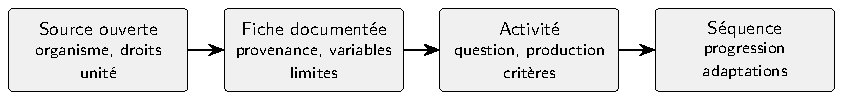
\includegraphics[width=13.4cm]{figures/flux-ressource-pedagogique.pdf}
\caption{Passage d'une source ouverte à une séquence pédagogique. Chaque flèche représente un travail d'explicitation et de vérification, non une simple conversion de format.}
\label{fig:flux}
\end{figure}

La reproductibilité intervient à chaque étape, mais elle ne signifie pas que toutes les données sont incorporées au dépôt. Certains scripts téléchargent une table officielle et écrivent les fichiers bruts et préparés dans des dossiers ignorés par Git. Ce choix limite la duplication de fichiers volumineux et évite de republier une donnée dont les droits ou la mise à jour relèvent de l'organisme source. Il déplace toutefois une responsabilité vers la préparation de séance : exécuter le script assez tôt, vérifier les colonnes attendues et conserver, lorsque cela est permis, un instantané daté pour le groupe. La fiche et l'activité doivent annoncer cette dépendance.

La version 0.1.0 utilise des catalogues générés à partir des métadonnées, plutôt qu'une liste saisie manuellement dans la page d'accueil. Les scripts de validation vérifient les champs obligatoires, la présence des fichiers, les liens entre une activité et son jeu de données, ainsi que les éléments du contrat pédagogique. Le site public expose aussi des aperçus limités pour certaines sources, sans confondre ces aperçus avec les données complètes. Ces mécanismes réduisent les divergences entre l'inventaire et le contenu. Ils ne garantissent pas qu'un portail externe restera disponible le jour d'un cours.

L'expression \og zéro déchet \fg~apparaît dans le projet comme une heuristique interne de conception. Elle invite à demander si une source assez riche peut soutenir plusieurs apprentissages au lieu d'être abandonnée après une seule démonstration. Les critères portent, entre autres, sur le contexte, la documentation, le nettoyage, la visualisation, la description, la modélisation, l'éthique et la réutilisation. Il ne s'agit ni d'un instrument validé ni d'une mesure environnementale. Un score élevé n'établit aucune efficacité pédagogique; il aide seulement l'équipe de conception à repérer les usages encore possibles et les limites à documenter.

Pour préparer une séance, une personne enseignante peut utiliser un protocole bref. Elle choisit d'abord une question compatible avec le temps disponible, puis ouvre la fiche pour vérifier l'unité, la source et la licence. Elle exécute le script ou place la table préparée dans le chemin annoncé. Elle produit elle-même le résultat minimal attendu. Elle décide ensuite ce qui sera fourni et ce qui devra être construit par les personnes étudiantes. Enfin, elle prépare une solution de repli : instantané daté, extrait autorisé ou résultat minimal, au cas où la source externe serait indisponible. Ce protocole transforme la reproductibilité en pratique d'enseignement plutôt qu'en simple propriété du code.

\section{Trois activités québécoises}

Les trois activités retenues couvrent une séance introductive, une étude de cas descriptive et un mini-projet de modélisation. Elles mobilisent respectivement un flux JSON opérationnel, une table démographique agrégée et un fichier administratif catégoriel. Le tableau~\ref{tab:activites} résume leurs contrastes; les paragraphes suivants détaillent les décisions de classe.

\begin{table}[ht]
\centering
\small
\begin{tabular}{p{2.8cm}p{3.2cm}p{3.2cm}p{3.2cm}}
\toprule
Activité & Données et niveau & Travail central & Production et limite principale \\
\midrule
BIXI, disponibilité instantanée & Flux GBFS JSON; introductif; 30 à 45 min & Jointure, ratio, distribution, stations vides & Graphique et interprétation; un instantané ne mesure pas la demande \\
\addlinespace
Structure d'âge Québec-Canada & Table StatCan; intermédiaire; 2 à 3 h & Filtrage, proportions, pyramides, comparaison temporelle & Rapport de 4 à 6 pages; description sans explication causale \\
\addlinespace
Gravité des accidents & Rapports policiers 2022; intermédiaire; 2 à 3 h & Recodage, description, modèle exploratoire, validation & Court rapport; association sans causalité ni risque sans exposition \\
\bottomrule
\end{tabular}
\caption{Trois activités de la version 0.1.0. Les durées et niveaux sont ceux du catalogue; ils doivent être adaptés au cours et au degré d'autonomie du groupe.}
\label{tab:activites}
\end{table}

\subsection{Décrire un instantané BIXI}

L'activité courte sur BIXI demande : \og Comment décrire la disponibilité des vélos BIXI dans un instantané? \fg~Elle s'appuie sur les flux GBFS de BIXI Montréal, recensés dans le portail Données Québec sous licence CC-BY 4.0 au moment de la vérification \cite{bixi}. L'unité après préparation est une station observée à un instant donné. Le script joint l'information relativement stable sur les stations et leur état instantané au moyen de \texttt{station\_id}. Cette définition de l'unité doit précéder tout calcul, car une ligne ne représente ni un trajet, ni une personne, ni une journée d'utilisation.

Les objectifs sont accessibles dans une introduction à la science des données : exécuter une importation JSON, comprendre une jointure, calculer un ratio avec un dénominateur pertinent, produire une distribution et nommer une limite. Les prérequis sont une première expérience des tables, des filtres et d'un graphique. Pour une séance de 30 à 45 minutes, l'enseignante ou l'enseignant prépare l'instantané avant le cours et vérifie le fichier \texttt{stations\_bixi\_snapshot.csv}. L'activité ne devrait pas dépendre d'un téléchargement en direct devant le groupe.

Le travail consiste à garder les stations de capacité positive, visualiser le taux d'occupation, calculer la proportion de stations sous un seuil de 25~\% et identifier celles qui n'ont aucun vélo disponible. La production attendue est un tableau ou un graphique accompagné de trois phrases d'interprétation prudente. La réussite ne se résume pas à un résultat numérique : la personne étudiante doit donner l'unité, justifier le dénominateur et éviter d'assimiler disponibilité, demande et qualité de service. Une station vide peut refléter des trajets, un rééquilibrage, une installation non active ou une combinaison de mécanismes que l'instantané ne permet pas de départager.

Une adaptation très courte fournit la table jointe et demande seulement le graphique, le calcul du seuil et une limite. Une adaptation avancée collecte des instantanés selon un horaire défini, documente leur horodatage et compare les changements. Cette variante exige un protocole de collecte, car interroger le flux de façon opportuniste ne produit pas une série temporelle représentative. La cartographie constitue une autre extension, à condition de filtrer les coordonnées invalides et de ne pas interpréter des points de station comme une mesure d'équité territoriale.

La version figée de l'activité est accessible dans le dépôt à l'adresse suivante : \href{https://github.com/AurelienNicosiaULaval/donnees-bleues/blob/v0.1.0/datasets/bixi/activite-courte.qmd}{activité BIXI, version 0.1.0}. Le lien vers l'étiquette protège la consigne contre les modifications ultérieures de la branche principale.

\subsection{Comparer la structure d'âge du Québec et du Canada}

La deuxième activité pose une question descriptive plus longue : \og Comment décrire l'évolution d'une structure démographique avec des données agrégées? \fg~Elle utilise le tableau 17-10-0005-01 de Statistique Canada, consacré aux estimations de population au 1er juillet par âge et genre \cite{statcan}. La source est annuelle, offerte sous la Licence ouverte de Statistique Canada et identifiable par un DOI. Après préparation, une ligne correspond à une combinaison d'année, de géographie, de catégorie de genre et de groupe d'âge.

Le mini-projet vise la statistique descriptive, la visualisation, la comparaison temporelle et la communication. Il convient à un groupe intermédiaire qui maîtrise l'importation d'un CSV, \texttt{dplyr} et les bases de \texttt{ggplot2}. L'enseignante ou l'enseignant exécute le script de préparation, vérifie les années disponibles et s'assure que les catégories de genre et les unités correspondent encore aux valeurs attendues. Le rapport compare le Québec et le Canada en proportions, car une comparaison des seuls effectifs confondrait structure et taille de population.

L'extrait suivant provient du code de départ de l'activité figée. Il charge explicitement les bibliothèques et rend visible la transformation signée utilisée uniquement pour dessiner les deux côtés d'une pyramide.

\begin{small}
\begin{verbatim}
library(dplyr)
library(ggplot2)
library(readr)
library(scales)

population_2025 <- read_csv(
  "data/processed/pyramides-ages/" |>
    paste0("population_pyramides_",
           "quebec_canada_latest.csv"),
  show_col_types = FALSE
)

ggplot(population_2025,
       aes(age_group, proportion_plot, fill = gender)) +
  geom_col(width = 0.85) +
  coord_flip() +
  facet_wrap(vars(geography)) +
  scale_y_continuous(
    labels = function(x) percent(abs(x), accuracy = 1)
  )
\end{verbatim}
\end{small}

La production attendue est un rapport Quarto de quatre à six pages comprenant la source, deux pyramides en proportions, un tableau de la part des 65 ans et plus en 2001 et en 2025, une comparaison Québec-Canada, les limites et le code reproductible. Les critères de réussite portent sur le filtrage explicite des années, géographies, genres, unités et groupes d'âge; sur l'explication de l'axe signé; et sur la séparation entre constat descriptif et interprétation causale. Les valeurs négatives de \texttt{proportion\_plot} servent à l'affichage et ne représentent évidemment pas une population négative.

Une version courte limite la tâche à une géographie et une année, fournit la table préparée et demande une pyramide annotée. Une version avancée ajoute une province ou une troisième année, mais oblige à harmoniser les catégories et à vérifier les révisions de la table. La source agrégée décrit une structure. Elle ne contient pas directement les naissances, les décès et les migrations nécessaires pour expliquer cette structure. Une conclusion sur les causes du vieillissement devrait donc mobiliser d'autres données et une autre activité.

La version figée est accessible ici : \href{https://github.com/AurelienNicosiaULaval/donnees-bleues/blob/v0.1.0/datasets/pyramides-ages/activite-longue.qmd}{structure d'âge, version 0.1.0}.

\subsection{Modéliser prudemment la gravité des accidents}

La troisième activité demande : \og Quels facteurs sont associés à la gravité des accidents, sans conclure trop vite à la causalité? \fg~Elle utilise les rapports d'accident remplis par les corps policiers et diffusés par la Société de l'assurance automobile du Québec dans Données Québec \cite{saaq}. Le fichier retenu pour l'activité couvre 2022 et comporte 108~186 rapports dans la ressource vérifiée. L'unité est un rapport d'accident, pas une personne exposée à la circulation. Cette nuance gouverne toute l'analyse.

Les objectifs sont de recoder des variables catégorielles documentées, présenter les distributions avant le modèle, définir une réponse binaire, ajuster un modèle exploratoire et communiquer les résultats comme des associations. Les prérequis sont une maîtrise de l'importation, des tableaux croisés et d'une régression logistique simple. Avant la séance, la personne enseignante exécute le script, vérifie le fichier préparé et consulte la documentation officielle des codes. Certaines variables utilisent la valeur 9 pour signifier \og trois ou plus \fg; additionner ces codes comme neuf victimes ou neuf véhicules produirait un résultat erroné.

Le travail commence par les valeurs manquantes et les catégories rares. Il se poursuit par un tableau descriptif selon la gravité, le mois, la météo et, au besoin, la région. Le modèle peut prendre \texttt{accident\_avec\_victime} comme réponse et employer le mois, la météo, la surface, l'éclairement et le type de jour comme variables explicatives. La production attendue est un court rapport reproductible avec contexte, tableau ou graphique, interprétation et limites. Un modèle réussi définit la réponse, décrit le traitement des valeurs manquantes, justifie les regroupements, distingue performance et interprétation, et ne transforme pas un coefficient en effet causal.

La limite centrale est l'absence de dénominateurs d'exposition. Le fichier ne contient pas le nombre de déplacements, la distance parcourue ou le volume de circulation correspondant à chaque condition. Une région comptant plus de rapports n'est pas nécessairement plus dangereuse; elle peut compter davantage de circulation ou une couverture différente. De même, une association entre météo et gravité dans les rapports ne mesure pas l'effet causal de la météo. Ces réserves ne sont pas un appendice défensif : elles déterminent la question statistique à laquelle le fichier peut répondre.

Une adaptation courte s'arrête aux tableaux croisés et à une proportion mensuelle. Une adaptation avancée compare des stratégies de validation, étudie séparément les accidents impliquant un vélo ou ajoute une donnée d'exposition documentée. Cette dernière option transforme réellement la question et nécessite une jointure dont la géographie, la période et l'unité doivent être compatibles. La version figée se trouve ici : \href{https://github.com/AurelienNicosiaULaval/donnees-bleues/blob/v0.1.0/datasets/rapports-accident/activite-longue.qmd}{rapports d'accident, version 0.1.0}.

\section{Composer une séquence d'enseignement}

Les trois activités peuvent être utilisées séparément, mais elles illustrent surtout une progression commune. Une première séance peut commencer avec BIXI : définir l'unité, joindre deux tables et discuter ce qu'un instantané permet de dire. Le mini-projet démographique ajoute la comparaison en proportions et une communication structurée. Le projet sur les accidents introduit ensuite le recodage, la validation et la distinction entre association, causalité et risque. La difficulté n'augmente pas seulement par la technique. Elle augmente par le nombre de décisions qu'il faut rendre explicites.

Une séquence de quatre rencontres peut conserver un même canevas. À la première rencontre, chaque groupe remplit une fiche de source : organisme, question de collecte, unité, période, géographie, licence et information absente. À la deuxième, il produit un tableau descriptif et une visualisation dont le titre nomme la population et la période. À la troisième, il formule deux conclusions, l'une acceptable et l'autre trop forte, puis explique la différence. À la quatrième, il remet un court document reproductible avec une section de limites. Ce canevas est transférable d'une source à l'autre et permet d'évaluer la qualité du raisonnement sans exiger le même résultat numérique.

Une même source peut aussi soutenir plusieurs gestes. Les rapports d'accident offrent un exemple complet. Le script importe les ressources officielles et nettoie les noms ou codes; l'activité courte explore des tableaux croisés et visualise des proportions; l'activité longue ajuste un modèle; le rapport communique les associations; la discussion finale nomme l'exposition absente et les limites causales. La continuité de la source permet de réinvestir le travail documentaire. Elle ne signifie pas qu'il faut forcer toutes les méthodes sur la même table. Si la question de modélisation exige une exposition qui n'existe pas, la bonne décision pédagogique peut être de s'arrêter ou de chercher une source complémentaire.

Pour une mise en oeuvre immédiate, l'enseignante ou l'enseignant peut choisir trois degrés de guidage. Dans une activité guidée, la table préparée, les variables et la structure du graphique sont fournies; l'effort porte sur l'unité et l'interprétation. Dans une étude de cas, le script de préparation est fourni, mais le choix du résumé et de la représentation appartient au groupe. Dans un projet, la question générale et les critères sont fixés, tandis que les personnes étudiantes justifient le nettoyage, la validation et les limites. Ces degrés peuvent coexister dans un même cours et faciliter l'adaptation à l'expérience en R.

Les critères d'évaluation gagnent à suivre le processus plutôt que la sophistication. Une production convaincante cite la source, nomme l'unité, conserve les transformations nécessaires, choisit un dénominateur cohérent, produit une représentation lisible, formule une conclusion proportionnée et identifie une information manquante. Un modèle complexe ne compense pas une unité mal définie. À l'inverse, une analyse descriptive simple peut démontrer une pensée statistique solide si elle relie correctement la question, la donnée et la portée du résultat.

\section{Limites, entretien et conditions d'utilisation}

Données bleues dépend de sources externes. Une adresse peut changer, un portail peut être indisponible, une API peut modifier son schéma et une catégorie peut être révisée. La date de consultation inscrite dans une fiche est donc une information substantielle. Avant chaque utilisation, il faut vérifier la source et, lorsque l'activité le permet, conserver un instantané autorisé. Un script qui échoue après une modification officielle n'invalide pas automatiquement l'idée pédagogique, mais il rend l'activité impropre à une séance tant que la préparation n'a pas été revue.

Les licences doivent être lues source par source. La présence d'un fichier sur un portail public ne signifie pas qu'il est sans conditions. Certaines données sont ouvertes avec attribution; d'autres sont seulement accessibles; des images peuvent relever de droits distincts. Données bleues renvoie vers l'organisme producteur et ne remplace pas ses conditions. Le dépôt ne possède pas, dans la version décrite, de licence générale qui aurait pour effet de relicencier les données tierces.

La proximité géographique ne garantit ni représentativité ni innocuité. Les données administratives sont produites par des processus de service, de déclaration ou d'enregistrement. Elles peuvent omettre des événements, refléter des différences de pratique ou rendre visibles de petits territoires. Une activité doit éviter les classements stigmatisants et les conclusions sur des groupes lorsque la source ne les soutient pas. Dans les exemples retenus, les limites sont intégrées aux critères de réussite précisément pour empêcher qu'elles soient reléguées à une phrase finale.

La reproductibilité comporte aussi une limite temporelle. Rejouer un script BIXI à une autre heure produit un autre instantané; rejouer une extraction StatCan après révision peut modifier les valeurs; télécharger un fichier annuel remplacé peut changer la structure. Une version figée du code ne fige pas nécessairement la donnée externe. Le dossier de cours devrait donc consigner le numéro de table ou de ressource, la date d'accès, l'horodatage lorsque pertinent et les sommes de contrôle des fichiers conservés localement.

Enfin, le statut documentaire des activités ne fournit aucune preuve sur leur usage. La version 0.1.0 ne permet pas de conclure que les données locales améliorent l'apprentissage, l'engagement ou la réussite. Une telle question exigerait un protocole distinct, une collecte appropriée et une analyse empirique. Le présent article se limite à une contribution de conception : rendre des activités concrètes, inspectables et adaptables. Les retours d'usage peuvent guider la maintenance, mais ils ne doivent pas être transformés en résultat de recherche sans cadre méthodologique et éthique adapté.

\section{Conclusion}

Enseigner avec des données québécoises ne consiste pas à remplacer les ressources internationales ni à décorer un exercice avec un nom de lieu. L'intérêt apparaît lorsque la provenance, l'unité, les catégories, les institutions et les limites deviennent une partie du raisonnement statistique. Données bleues propose une infrastructure éditoriale simple pour effectuer ce travail : partir d'une source officielle, documenter ce qu'elle mesure, construire une activité autour d'une question et rendre la portée du résultat vérifiable.

Les exemples BIXI, démographie et accidents montrent trois niveaux d'engagement avec les données. Ils vont d'un instantané descriptif à une comparaison structurale, puis à une modélisation exploratoire. Dans chaque cas, la production attendue associe un résultat à une limite. C'est cette association, plus que la localisation de la donnée, qui constitue la proposition pédagogique centrale.

La version 0.1.0 rend les activités accessibles et citables. Leur prochaine étape appartient aux usages documentés : adaptation à des cours précis, vérification avant chaque séance, révision des sources et, si une évaluation empirique est entreprise, distinction nette entre expérience d'enseignement et preuve de recherche. Le Québec fournit ici un contexte riche. La rigueur vient du soin avec lequel on apprend à le lire dans les données.

\bigskip
\begin{thebibliography}{10}
\raggedright

\bibitem{bixi} BIXI Montréal et Données Québec (s.d., consultation le 23 août 2026). \emph{État des stations BIXI}. Gouvernement du Québec. \url{https://www.donneesquebec.ca/recherche/dataset/vmtl-bixi-etat-des-stations}

\bibitem{finch} Finch, S. et Gordon, I. (2023). Bare bones, or a rich feast? Taking care with context in a data rich world, \emph{Teaching Statistics, 45}(1), 4--13. \url{https://doi.org/10.1111/test.12322}

\bibitem{gaise} GAISE College Report ASA Revision Committee (2016). \emph{Guidelines for Assessment and Instruction in Statistics Education: College Report 2016}. American Statistical Association. \url{https://www.amstat.org/asa/files/pdfs/GAISE/GaiseCollege_Full.pdf}

\bibitem{gould} Gould, R. (2017). Data literacy is statistical literacy, \emph{Statistics Education Research Journal, 16}(1), 22--25. \url{https://doi.org/10.52041/serj.v16i1.209}

\bibitem{donneesbleues} Nicosia, A. (2026). \emph{Données bleues} (version 0.1.0) [plateforme pédagogique et code source]. \href{https://github.com/AurelienNicosiaULaval/donnees-bleues/releases/tag/v0.1.0}{Publication GitHub de la version 0.1.0}.

\bibitem{saaq} Société de l'assurance automobile du Québec et Données Québec (s.d., consultation le 23 août 2026). \emph{Rapports d'accident}. Gouvernement du Québec. \url{https://www.donneesquebec.ca/recherche/dataset/rapports-d-accident}

\bibitem{statcan} Statistique Canada (2025). \emph{Estimations de la population au 1er juillet, par âge et genre}, tableau 17-10-0005-01. \url{https://doi.org/10.25318/1710000501-fra}

\bibitem{unesco} UNESCO (2019). \emph{Recommandation sur les ressources éducatives libres}. Paris, France : UNESCO. \url{https://www.unesco.org/fr/legal-affairs/recommendation-open-educational-resources-oer}

\bibitem{wild} Wild, C. J. et Pfannkuch, M. (1999). Statistical thinking in empirical enquiry, \emph{International Statistical Review, 67}(3), 223--248. \url{https://doi.org/10.1111/j.1751-5823.1999.tb00442.x}

\bibitem{wright} Wright, C., Meng, Q., Breshock, M. R., Atta, L., Taub, M. A., Jager, L. R., Muschelli, J. et Hicks, S. C. (2024). Open Case Studies: Statistics and data science education through real-world applications, \emph{Journal of Statistics and Data Science Education, 32}(4), 331--344. \url{https://doi.org/10.1080/26939169.2024.2394541}

\end{thebibliography}


\end{document}
